\documentclass[pdftex]{beamer}

\setbeamertemplate{navigation symbols}{} % выключить навигационную панльку
\setbeamertemplate{footline}[frame number] % нумерация страниц

\usepackage{graphicx}
\usepackage{amsmath,amssymb,amsthm}
\usepackage{pb-diagram}
\usepackage{ucs}
\usepackage[utf8x]{inputenc}
\usepackage[russian]{babel}
\usepackage{epstopdf}
\usepackage{multicol}
\usepackage{cancel}
\usepackage{hyperref}
\usepackage{amsfonts}

\usepackage{listings}
\usepackage{textcomp}
\definecolor{listinggray}{gray}{0.9}
\definecolor{lbcolor}{rgb}{0.9,0.9,0.9}
\lstset{
  %	backgroundcolor=\color{lbcolor},
  language=Mathematica,
  tabsize=2,
  rulecolor=,
  basicstyle=\scriptsize,
  upquote=true,
  % aboveskip={1.5\baselineskip},
  columns=fixed,
  showstringspaces=false,
  extendedchars=true,
  % breaklines=true,
  prebreak = \raisebox{0ex}[0ex][0ex]{\ensuremath{\hookleftarrow}},
  % frame=single,
  showtabs=false,
  showspaces=false,
  showstringspaces=false,
  identifierstyle=\ttfamily,
  keywordstyle=\color[rgb]{0,0,1},
  commentstyle=\color[rgb]{0.133,0.545,0.133},
  stringstyle=\color[rgb]{0.627,0.126,0.941},
}

%%%%%%%%%%%%%%%%%%%%%%%%%%%%%%%%%%%%%%%%%%%%%%%%%%%%%%%%%%%%%%%%%%%%%%%%%%%%%%%%%%%%%%%%%%%%%%%%%%% 
\newtheorem{Sl}{Corollary}
\newtheorem{Utv}{Proposition}
%% \newtheorem{acknowledgement}[theorem]{Acknowledgement}
%% \newtheorem{algorithm}[theorem]{Algorithm}
%% \newtheorem{axiom}[theorem]{Axiom}
%% \newtheorem{case}[theorem]{Case}
%% \newtheorem{claim}[theorem]{Claim}
%% \newtheorem{conclusion}[theorem]{Conclusion}
%% \newtheorem{condition}[theorem]{Condition}
%% \newtheorem{conjecture}[theorem]{Conjecture}
%% \newtheorem{mycorollary}[theorem]{Corollary}
%% \newtheorem{mycriterion}[theorem]{Criterion}
%% \newtheorem{mydefinition}[theorem]{Definition}
%% \newtheorem{myexample}[theorem]{Example}
%% \newtheorem{myexercise}[theorem]{Exercise}
\newtheorem{mylemma}[theorem]{Лемма}
%% \newtheorem{mynotation}[theorem]{Notation}
%% \newtheorem{myproblem}[theorem]{Problem}
%% \newtheorem{myproposition}[theorem]{Proposition}
%% \newtheorem{myremark}[theorem]{Remark}
%% \newtheorem{mysolution}[theorem]{Solution}
%% \newtheorem{mysummary}[theorem]{Summary}
%% \newenvironment{myproof}[1][Proof]{\textbf{#1.} }{\ \rule{0.5em}{0.5em}}


\newcommand{\go}{\stackrel{\circ }{\mathfrak{g}}}
\newcommand{\ao}{\stackrel{\circ }{\mathfrak{a}}}
\newcommand{\co}[1]{\stackrel{\circ }{#1}}
\newcommand{\pia}{\pi_{\mathfrak{a}}}
\newcommand{\piab}{\pi_{\mathfrak{a}_{\bot}}}
\newcommand{\gf}{\mathfrak{g}}
\newcommand{\gfh}{\hat{\mathfrak{g}}}
\newcommand{\af}{\mathfrak{a}}
\newcommand{\afh}{\hat{\mathfrak{a}}}
\newcommand{\bff}{\mathfrak{b}}
\newcommand{\afb}{\mathfrak{a}_{\bot}}
\newcommand{\hf}{\mathfrak{h}}
\newcommand{\hfg}{\hf_{\gf}}
\newcommand{\hfb}{\mathfrak{h}_{\bot}}
\newcommand{\pf}{\mathfrak{p}}
\newcommand{\aft}{\widetilde{\mathfrak{a}}}
\newcommand{\sfr}{\mathfrak{s}}
% \pagestyle{plain}

\theoremstyle{definition} \newtheorem{Def}{Definition}
\setbeamertemplate{caption}[empty]
\newcommand{\tr}{\hat\triangleright} \newcommand{\trc}{\triangleright}
\newcommand{\adk}{a^{\dagger}_{\kappa}} \newcommand{\ak}{a_{\kappa}}
\def\bF{\mbox{$\overline{\cal F}$}} \def\F{\mbox{$\cal F$}}

\usetheme{AnnArbor}
% \usetheme{Warsaw}


\title[Special splints]{Splints of root systems for special Lie subalgebras}

\author[Kakin, Lyakhovsky, Nazarov]{Polina Kakin, Vladimir Lyakhovsky, \underline{Anton Nazarov}}


\institute[SPbSU]{
  Department of High Energy and Elementary Particle Physics\\
  Physical faculty\\
  SPSU\\
}

\date[Novozhilov's 90] % (optional, should be abbreviation of conference name)
{In Search of Fundamental Symmetries
  \\December 2014}
\begin{document}

%% Plan:
%% 1. Structure of irrep is defined by additive properties of root system (Verma module+singular element = Weyl formula)
%% 2. Non angle-preserving map, splint
%% 3. Classification of splints, statement
%% 4. Special embeddings
%% 5. Projection of root system: examples
%% 6. Classification, Dynkin diagrams with multiplicities
%% 7. Conclusion
%% 
\maketitle
\section{Introduction}
\begin{frame}
  \frametitle{Root systems and irreducible representations}
  \begin{itemize}
  \item Additive properties of root system determine Verma module
    \begin{equation*}
      M^{\mu}=U(\gf)\underset{U(\bff_{+})}{\otimes} D^{\mu}(\bff_{+})=\{(E^{-\alpha_{1}})^{n_{1}}\dots (E^{-\alpha_{s}})^{n_{s}} \left|v_{\mu}\right>\}_{\alpha_{i}\in\Delta^{+}}^{n_{i}=0,1,\dots}
    \end{equation*}
    \begin{figure}[h]
      \center{\includegraphics[width=0.4\linewidth]{B2_Verma}}
      \vspace{-0.3cm}
      \caption{Verma module and root system of $B_{2} (so(5))$ Lie algebra} 
      \label{verma}
    \end{figure}
    \vspace{-0.3cm}
  \item Weyl formula: singular element and characters of Verma modules
    \begin{equation*}
      \mathrm{ch} L^{\mu}=\frac{\sum_{w\in W} \epsilon(w) e^{w(\mu+\rho)-\rho}}{\sum_{w\in W}\epsilon(w) e^{w\rho-\rho}}=\sum_{w\in W} \epsilon(w)\; \mathrm{ch} M^{w(\mu+\rho)-\rho}
    \end{equation*}

    
  \end{itemize}
\end{frame}
\begin{frame}
  \frametitle{Splint of a root system}
  Idea: consider root systems up to non-angle-preserving maps $\iota:\tilde\Delta\to \Delta$, $\iota(\alpha)=\iota(\alpha_{1})+\iota(\alpha_{2})\Leftrightarrow \alpha=\alpha_{1}+\alpha_{2}$

  A root system $\Delta$ "splinters"{ }as $\left(\Delta_{\af},\Delta_{\sfr}\right)$ if there are two embeddings $\iota_1:\Delta_{\af}\hookrightarrow\Delta$ and $\iota_2:\Delta_{\sfr}\hookrightarrow\Delta$.      $\Delta_{\af}$, $\Delta_{\sfr}$ are the "stems"{ }of the splint.

  % where $\left(a\right)$ $\Delta$ is a disjoint union of the images of $\iota_1$ and $\iota_2$ $\left(b\right)$ neither the rank of $\Delta_1$ nor the rank of $\Delta_2$ exceeds the rank of~$\Delta$.

  \begin{equation*}
    \begin{array}{cc||c|c}
      \hbox{type} & \hspace{0.25in}\Delta \hspace{0.25in} & \hspace{0.25in}\Delta
      _{\frak{a}}\hspace{0.25in} & \hspace{0.25in}\Delta _{\frak{s}}\hspace{0.25in}
      \\ \hline\hline
      \hbox{(1)} & G_{2} & A_{2} & A_{2} \\
      & F_{4} & D_{4} & D_{4} \\ 
      & B_{2} & D_{2} & D_{2} \\ \hline
      \hbox{(2)} & B_{r}(r\geq 3) & D_{r} & \oplus ^{r}A_{1} \\
      (*)& C_{r}(r\geq 3) & \oplus ^{r}A_{1} &  D_{r} \\ \hline
      \hbox{(3)} & A_{r}(r\geq 2) & A_{r-1}\oplus u\left( 1\right)  & \oplus
      ^{r}A_{1} \\
      & B_{2} & A_{1}\oplus u\left( 1\right)  & A_{2}
    \end{array}
    \label{tb2}
  \end{equation*}

  Reduction $\gf\downarrow \af$: \quad$\pi\left(\mathrm{ch}L^{\mu}_{\gf}\right)=\sum_{\nu} b^{(\mu)}_{\nu} \mathrm{ch}L^{\nu}_{\af}$
\end{frame}

\begin{frame}
  \frametitle{Branching coefficients $=$ weight multiplicities of $\mathfrak{s}$}
  
  \begin{figure}[h!bt]
    \noindent\centering{
      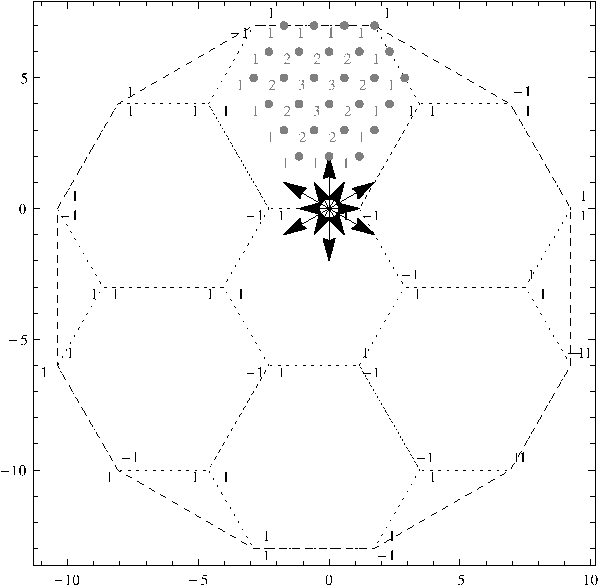
\includegraphics[width=40mm]{g2}
    }\vspace{-0.3cm}
    \caption{Weyl group orbit  (long dash) for  $\Psi_{G_{2}}(L^{[3,2]})$ and its decomposition into sum of images of singular elements of   $A_{2}$ modules (short dash). Weight multiplicities of  $L^{[3,2]}_{A_{2}}$ coincide with branching coefficients $L^{[3,2]}_{G_{2}\downarrow A_{2}}$.}
    \label{fig:g2_splint}
  \end{figure}\vspace{-0.3cm}
  \begin{equation*}
    b_{(\mu-\iota (\tilde{\mu}-\tilde{\nu}))}^{(\mu)}=M_{\sfr (\tilde{\nu})}^{(\tilde{\mu})}, 
  \end{equation*}

  $M^{(\tilde\mu)}_{\sfr(\tilde\nu)}$ - the multiplicity of the weight $\tilde\nu$ in the module $L^{\tilde\mu}_{\sfr}$ of algebra $\sfr$,\\
  $\tilde\mu=\sum m_k \tilde\omega_k$,  $\tilde\omega_k$ - fundamental weights for $\sfr$, $m_k$ - Dynkin labels of $\mu$.
\end{frame}
\section{Special subalgebras}
\begin{frame}
  \frametitle{Splint in the case of special embedding}
  \begin{Def}
    Embedding $\af \rightarrow \gf $ of semisimple Lie algebras is called "special"{ }if a root system $ \Delta _ {\af} $ of algebra $ \af $ is not a subsystem of a root system $ \Delta _ {\gf} $ of algebra $ \gf $.
  \end{Def}
  To construct an embedding consider some representation $L^{\mu}_{\af}$ as a subspace of Lie algebra $\gf$. Get generators of $\af$ as linear combinations of generators of $\gf$. To reduce $\gf$-representations project $\gf$ root system to Cartan subalgebra of $\af$. 

  Properties of special subalgebras \cite {d}
  \begin{itemize}
  \item Orthogonal projection of algebra $\gf$ onto root space of subalgebra $\af$ contains a root system of subalgebra $\af$ 
  \item Projections of the roots of algebra $\gf$ are linear combinations of the roots of subalgebra $\af$ with integer coefficients.
  \end{itemize}
\end{frame}


\begin{frame}
  \frametitle{Orthogonal projection and splint}
  \begin{itemize}
  \item $\Delta'$ is orthogonal projection of the root system $\Delta_{\gf}$ onto the root space of subalgebra $\af$
    \begin{itemize}
    \item $\Delta'\supset\Delta_{\af}$
    \item $\Delta'$ contains some roots of $\Delta_{\af}$ more than once
    \end{itemize}
  \item $\Phi_{\gf}^{(\mu)'}$ is orthogonal projection of the singular element of $\gf$-representation  onto the root space of subalgebra $\af$ 
  \item $\Delta'\approx\left(\Delta_{\af},\Delta_{\sfr}\right)$ is a special splint
  \item $\Delta_{\sfr}=\Delta' \backslash \Delta_{\af}$ is a system of vectors
  \item $W_{\sfr}$ is a group of reflections in hyperplanes orthogonal to the vectors in $\Delta_{\sfr}$
  \item $W_{inv}$ is a group of reflections in hyperplanes orthogonal to the roots from $\Delta_{\gf}$ that already lie in the root space of subalgebra $\af$.
  \end{itemize}
\end{frame}

\begin{frame}
  \frametitle{Examples of root system projections}
  \begin{multicols}{4}
    \begin{figure}[h!tb]
      \includegraphics[width=1.0\linewidth]{Special-A1-A1-A3}      
      \caption{$A_1+A_1\to A_3$}
      \label{fig:a1a1a3}
    \end{figure}
    \begin{figure}[h!tb]
      \includegraphics[width=1.0\linewidth]{Special-A2-A5}      
      \caption{$A_2\to A_5$}
      \label{fig:a2a5}
    \end{figure}
    \begin{figure}[h!tb]
      \includegraphics[width=1.0\linewidth]{Special-A2-D4}
      \caption{$A_2\to D_4$}
      \label{fig:a2d4}
    \end{figure}
    \begin{figure}[h!tb]
      \includegraphics[width=1.0\linewidth]{Special-G2-B3}      
      \caption{$G_2\to B_3$}
      \label{fig:g2b3}
    \end{figure}
    
  \end{multicols}

\end{frame}

\section{Types of special splints}
%% \begin{frame}
%%   \frametitle{Special splints: $\Delta_s\subset\Delta_a$}
%%   \begin{Utv}
%%     If $\Delta'\approx\left(\Delta_a,\Delta_s\right)$ is a special splint and $\Delta_s\subset\Delta_a$ then:
%%     
%%     $$
%%     \Phi_g^{(\mu)'}=\sum_{w\in W_{inv}} \epsilon (w) w(1+\sigma_1+\dots)(e^{\hat\mu+\hat\rho_g-\tilde{\mu}-\tilde{\rho_s}}\Phi_s^{(\tilde{\mu})}),
%%     $$
%%     \begin{itemize}
%%     \item where $\sigma_1+\dots$ are elements of the group $W_s$ that move $\Phi_s^{(\tilde{\mu})}$ to the next Weyl chamber of subalgebra $a$. The number of elements is equal to the number of the fundamental Weyl chamber of subalgebra $a$ one needs to fill the fundamental Weyl chamber of the group $W_{inv}$. 
%%       
%%     \item The vector $\hat\mu+\hat\rho_g$ is vector of the highest lenght in the projection of the singular element $\Phi_g^{(\mu)'}$ with positive multiplicity.
%%     \end{itemize}
%%     \label{u3}
%%   \end{Utv}
%% \end{frame}
%% 
%% \begin{frame}
%%   \frametitle{Special splints: $\Delta_a\subset\Delta_s$}
%%   \begin{Utv}
%%     If $\Delta'\approx\left(\Delta_a,\Delta_s\right)$ is a special splint and $\Delta_a\subset\Delta_s$ while $W_{inv}\subset\Delta_a$ then:
%%     
%%     $$
%%     \Phi_g^{(\mu)'}=\sum_{w\in W_{inv}} \epsilon (w) w(1+\sigma_1+\dots)(e^{\hat\mu+\hat\rho_g-\tilde{\mu}-\rho_s}\Phi_s^{(\tilde{\mu})});
%%     $$
%%     if there is no $W_{inv}$ or $W_{inv}\not\subset W_a$ then:
%%     $$
%%     \Phi_g^{(\mu)'}=(2-\sum_{w\in W_a} \epsilon (w) w)(e^{\hat\mu+\hat\rho_g-\tilde{\mu}-\rho_s}\Phi_s^{(\tilde{\mu})}).
%%     $$
%%     \label{u2}
%%   \end{Utv}
%% \end{frame}
%% 

\begin{frame}
  \frametitle{Types of special splints}
  \begin{table}[h]
    \begin{tabular}[t]{|p{1,5em}|p{5em}|p{5em}|p{5em}|p{2em}|p{6em}|}
      \hline
      Type & $s$ & $W_{\af}\subset W_{\sfr}$ & $W_{\sfr}\subset W_{\af}$ & $W_{inv} $ & Examples \\
      \hline
      1 & root system & no & yes & yes  & $B_2\rightarrow D_3$, $G_2\rightarrow B_3$\\
      \hline
      2 & root system & yes & yes & no & $A_1\rightarrow A_1+A_1$ \\
      \hline
      3 & root system & yes & yes & no & $A_1+A_1\rightarrow D_3$ \\
      \hline
      4 & not a root system & yes & no & yes & $A_1\rightarrow A_2$, $A_1\rightarrow B_3$\\
      \hline
      5 & not a root system & yes & no & no  & $A_1\rightarrow B_2$\\
      \hline
      6 & \multicolumn{4}{|l|}{$W_{\af}\not\subset W_{\sfr}$ and $W_{\sfr}\not\subset W_{\af}$} & $B_2\rightarrow D_4$\\
      \hline
    \end{tabular}
    \label {spsp}
    In first three cases coincidence of branching coefficients with weight multiplicities of $\sfr$-representations takes place. 
  \end{table}
\end{frame}

%%   \begin{frame}
%%     \frametitle{Special splints and branching coefficients}
%%     \begin{Sl}
%%       If $\Phi_s^{(\tilde{\mu})}$ can be put in the fundamental Weyl chamber $\bar C_a$ of subalgebra $a$ then by applying injection fan to the singular element $\Phi_s^{(\tilde{\mu})}$ one obtains $M_{s (\tilde{\nu})}^{(\tilde{\mu})}=b_{(\mu-\tilde{\mu}+\tilde{\nu})}^{(\mu)}$. If $\Phi_s^{(\tilde{\mu})}$ can not be put in $\bar C_a$ then $b_{(\mu-\tilde{\mu}+\tilde{\nu})}^{(\mu)}=N_{(\tilde{\nu})}$ where $N_{(\tilde{\nu})}$ are as follows: $$V_{a\rightarrow g}^{-1}(1+\sigma_1+\dots)(e^{\hat\mu+\hat\rho_g-\tilde{\mu}-\rho_s}\Phi_s^{(\tilde{\mu})}))=\sum_{\tilde{\nu}} N_{(\tilde{\nu})}e^{\tilde{\mu}}.$$
%%       In both cases $\tilde{\nu}\in\bar C_a$ and the fundamental Weyl chamber $\bar C_a$ begins in the point $\tilde{\mu}-\mu$.
%%       \label{u31}
%%     \end{Sl}
%% 
%% 
%%   \end{frame}
%% 
%% 




\section{Examples}

\begin{frame}
  \frametitle{Splint for embedding $B_2\rightarrow D_3$ ($so(5)\rightarrow so(6)$)}


  \begin{figure}[h]
    \center{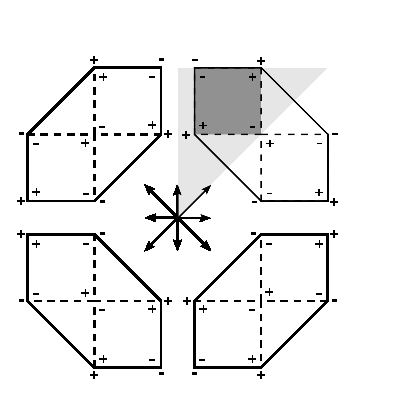
\includegraphics[width=0.4\linewidth]{drawing-1}}
    \caption{Splint $D_3\approx (B_2,A_1+A_1)$: projection of the singular element $\Phi_{D_3}^{([1,1,2])'}$ can be made from singular elements $\Phi_{A_1+A_1}^{([1,1])}$. Light-grey area is the fundamental Weyl chamber of subalgebra $B_2$.} 
    \label{ris3}
  \end{figure}
\end{frame}

\begin{frame}
  \frametitle{Splint for embedding $B_2\rightarrow D_3$ ($so(5)\rightarrow so(6)$)}


  \begin{figure}[h]
    \center{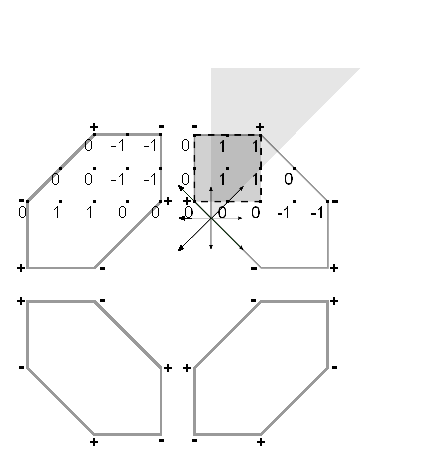
\includegraphics[width=0.4\linewidth]{drawing-3}}
    \caption{Injection fan applied to the singular element $\Phi_{A_1+A_1}^{([1,1])}$ yields branching coefficients that are equal to 1 which is in agreement with the Gelfand-Tzeytlin rule for branching for embeddings $so(2n-1)\rightarrow so(2n)$. }
    \label{ris5}
  \end{figure}


\end{frame}

\begin{frame}
  \frametitle{Splint for embedding $G_2\rightarrow B_3$ ($g(2)\rightarrow so(7)$)}

  \begin{figure}[h]
    \center{\includegraphics[width=0.5\linewidth]{drawing-4}}
    \caption{Splint $B_3\approx (G_2,A_2)$: projection of the singular element $\Phi_{B_3}^{([0,0,1])'}$ can be made from singular elements $\Phi_{A_2}^{([0,1])}$. Light-grey area is the fundamental Weyl chamber of subalgebra $G_2$.}
    \label{ris6}
  \end{figure}


\end{frame}

\begin{frame}
  \frametitle{Splint for embedding $A_1\rightarrow A_2$ ($so(3)\rightarrow su(3)$)}

  \begin{figure}[h]
    \center{\includegraphics[width=0.7\linewidth]{drawing-5}}
    \label {a5}
    \caption{Projection of the singular element $\Phi_{A_2}^{([1,1])'}$ can be made from two singular elements $\Phi_{BC_1}^{(\tilde{\mu})}$.}
  \end{figure}


\end{frame}

\begin{frame}
  \frametitle{Splint for embedding $A_1+A_1\rightarrow D_3$ ($so(4)\rightarrow so(6)$)}

  \begin{figure}[h]
    \center{\includegraphics[width=0.4\linewidth]{drawing-2}}
    \caption{Splint $D_3\approx (A_1+A_1,B_2)$: projection of the singular element $\Phi_{D_3}^{([1,1,2])'}$ can be made from singular elements $\Phi_{B_2}^{([1,2])}$ (one of them is marked with grey colour).}
    \label{ris4}
  \end{figure}


\end{frame}

\section{Conclusion}

\begin{frame}
  \frametitle{Towards classification of splints for special embeddings}
  \begin{itemize}
  \item Number of special embeddings is infinite: arbitrary algebra $\gf$, $\af$-representation
  \item Splints are rare
  \item We can use Dynkin diagrams with multiplicities for projections
  \item Diagrams of the same rank as $\af$ should be considered, root multiplicities less or equal to 2
  \end{itemize}
\vspace{-0.3cm}
  \begin{multicols}{4}
    \begin{figure}[h!tb]
      \includegraphics[width=1.0\linewidth]{Special-A1-A1-A3}      \\
      \includegraphics[width=0.8\linewidth]{A1A1A3}      
      \caption{$A_1+A_1\to A_3$}
      \label{fig:a1a1a3}
    \end{figure}
    \begin{figure}[h!tb]
      \includegraphics[width=1.0\linewidth]{Special-A2-A5}      \\
      \includegraphics[width=0.8\linewidth]{A2A5}      \vspace{-0.3cm}
      \caption{$A_2\to A_5$}
      \label{fig:a2a5}
    \end{figure}\par
    \begin{figure}[h!tb]
      \includegraphics[width=1.0\linewidth]{Special-A2-D4}\\
      \includegraphics[width=0.8\linewidth]{A2D4}      
      \caption{$A_2\to D_4$}
      \label{fig:a2d4}
    \end{figure}
    \begin{figure}[h!tb]
      \includegraphics[width=0.8\linewidth]{Special-G2-B3}      \\
      \includegraphics[width=0.8\linewidth]{G2B3}      \vspace{-0.2cm}
      \caption{$G_2\to B_3$}
      \label{fig:g2b3}
    \end{figure}
    
  \end{multicols}

\end{frame}
\section{Conclusion}


\begin{frame}
  \frametitle{Conclusion}
  \begin{itemize}
  \item The concept of splint was generalised on the case of special embedding.
  \item The way to simplify calculation of branching coefficients was found for the case when both stems are root systems.
  \item Some generalization of Dynkin diagrams can be useful. 
  \end{itemize}

\end{frame}

\begin{frame}
  \frametitle{References}
  \begin{thebibliography}{99}

  \bibitem{ln}
    {\it V.D.Lyakhovsky, A.A.Nazarov}
    Fan, splint and branching rules.
    // Зап. научн. сем. ПОМИ, т. 398, стр. 162–178 (2012)
    arXiv:1111.6787v2 (2011)

  \bibitem{b1}
    {\it V.D.Lyakhovsky, S.Melnikov, er al}
    Recursion relations and branching rules for simple Lie algebras.
    // Journal of Physics A-Mathematical and General 29, no. 5, p.1075-1088 (1996)

  \bibitem{b2}
    {\it V.D.Lyakhovsky, A.A.Nazarov}
    Recursive algorithm and branching for nonmaximal embeddings.
    // Journal of Physics A-Mathematical and General 44, no. 7 (2011)

  \bibitem{sp1}
    {\it D.V.Vasilevich, V.D.Lyakhovsky}
    Method of special embeddings for grand unification models.
    // Theoretical and Mathematical Physics, 66:3, p. 231–237 (1986)

  \bibitem{d}
    {\it Е.Б.Дынкин}
    Полупростые подалгебры полупростых алгебр.
    // Тр. Моск. матем. об-ва, т.1, стр. 39-166 (1952)

  \end{thebibliography}
\end{frame}

\begin{frame}[c]
  \begin{center}
    \Large{Thank you for attention!}    
  \end{center}

  %% \begin{figure}[h]
  %%   \center{\includegraphics[width=0.65\linewidth]{IMG_1777}}
  %%   
  %% \end{figure}
  %% 


\end{frame}

\end{document}
